\documentclass[main]{subfiles}
\begin{document}

\subsection{管理者専用機能}
\subsubsection{管理者専用機能TOP画面}
図\ref{fig:TOP2}に管理者専用機能TOP画面を示す.機能をクリックするとそれぞれの機能画面に遷移する.総合TOPに戻るをクリックすると図\ref{fig:TOP1}に遷移する.

\begin{figure}[H]
 \centering
   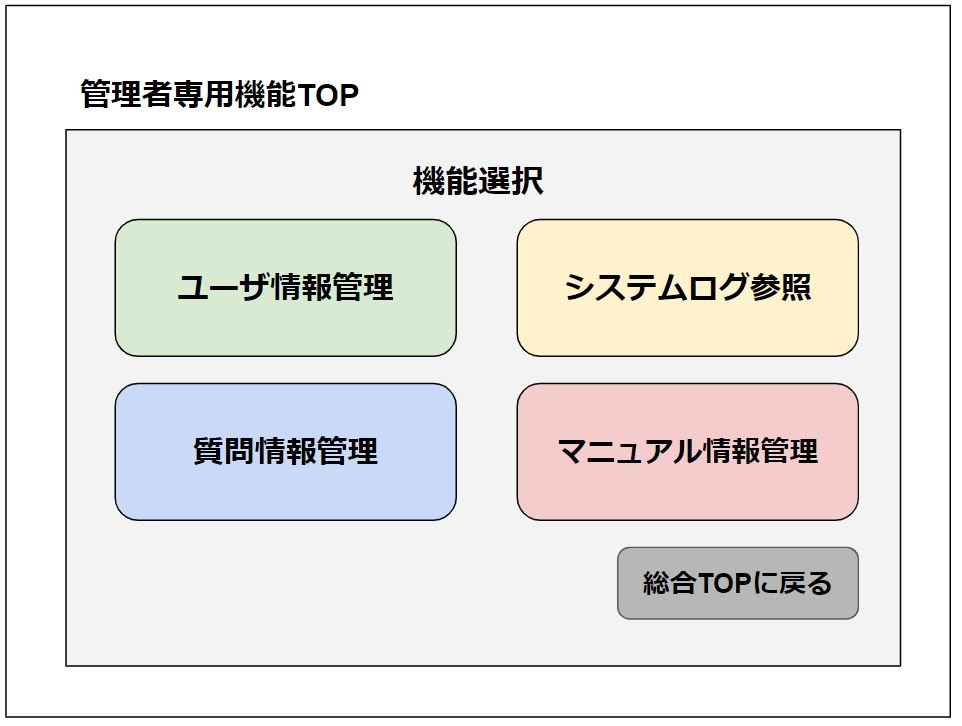
\includegraphics[width=100mm]{UI-umino/TOP2.JPG}
 \caption{管理者専用機能TOP画面}
 \label{fig:TOP2}
\end{figure}

\subsubsection{ユーザ情報管理画面}
図\ref{fig:user1}にユーザ情報管理画面を示す.ユーザ情報管理画面ではユーザID,ユーザ名,最終ログインを確認することができる.

\begin{figure}[H]
 \centering
   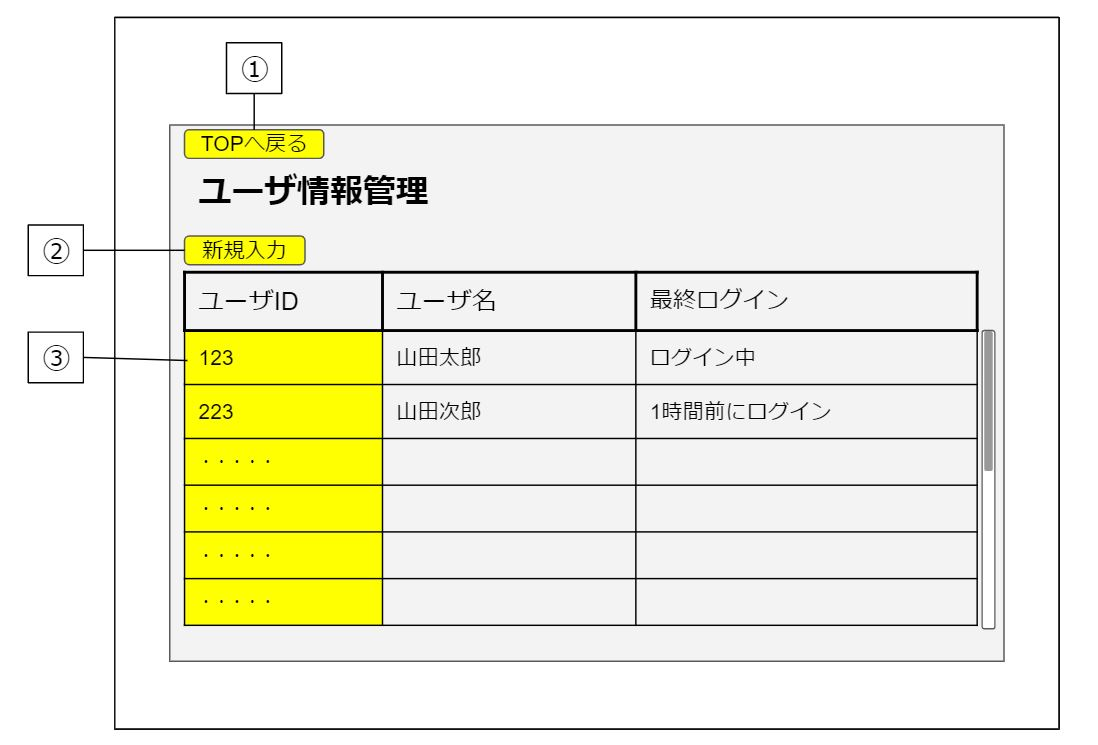
\includegraphics[width=100mm]{UI-umino/user1.JPG}
 \caption{ユーザ情報管理画面}
 \label{fig:user1}
\end{figure}

\begin{enumerate}
\renewcommand{\labelenumi}{\textcircled{\scriptsize \theenumi}}
\item TOPへ戻る\\ クリックすることで図\ref{fig:TOP1}に遷移する.
\item 新規入力\\ ユーザ情報の新規入力を行う際には,クリックすることで図\ref{fig:user2}に遷移する.
\item ユーザID\\ 表示されたユーザIDをクリックすることで図\ref{fig:user3}に遷移し,クリックしたユーザの情報を編集,削除することができる.
\end{enumerate}

\subsubsection{ユーザ情報入力・編集画面}
図\ref{fig:user2}に新規ユーザ情報入力画面,図\ref{fig:user3}にユーザ情報編集画面を示す.ユーザIDには指定範囲内の任意の数字の組み合わせを使用できる.ユーザ名には本名を入力する.パスワードは,使用するユーザが設定する.ユーザ権限は,使用するユーザによって必要になる権限にチェックを入れることで権限を得ることができる.取消をクリックすることで図\ref{fig:user1}に戻る.登録をクリックすることで図\ref{fig:user4}へ,削除をクリックすることで図\ref{fig:user5}にそれぞれ遷移する.

\begin{figure}[H]
    \begin{minipage}{0.5\hsize}
        \centering
        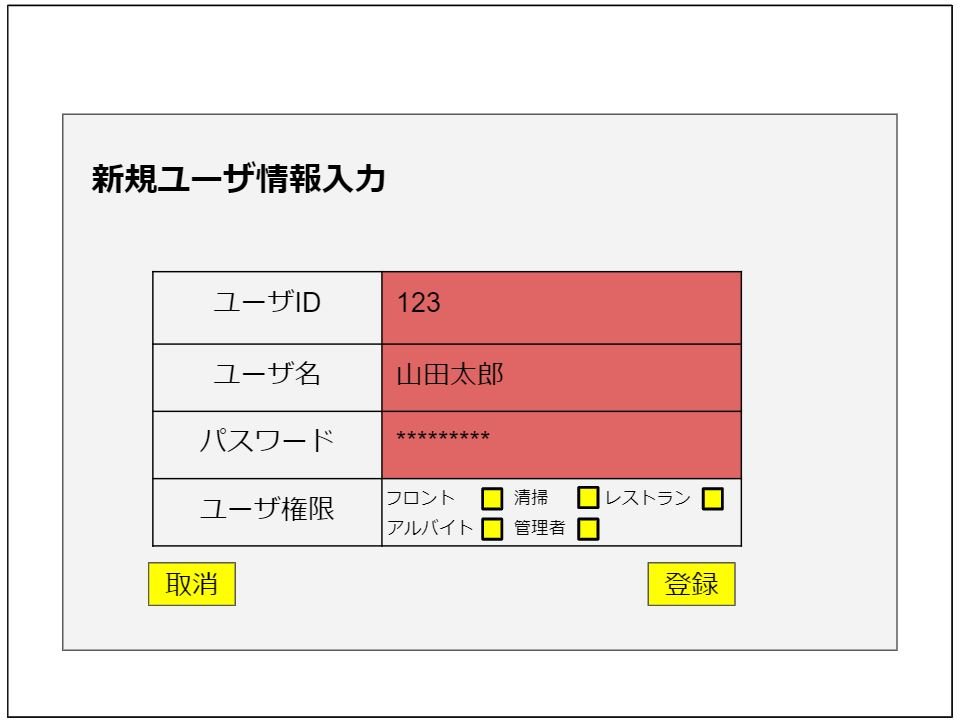
\includegraphics[width=7cm]{UI-umino/user2.JPG}
        \caption{新規ユーザ情報入力画面}
        \label{fig:user2}
    \end{minipage}
    \begin{minipage}{0.5\hsize}
        \centering
        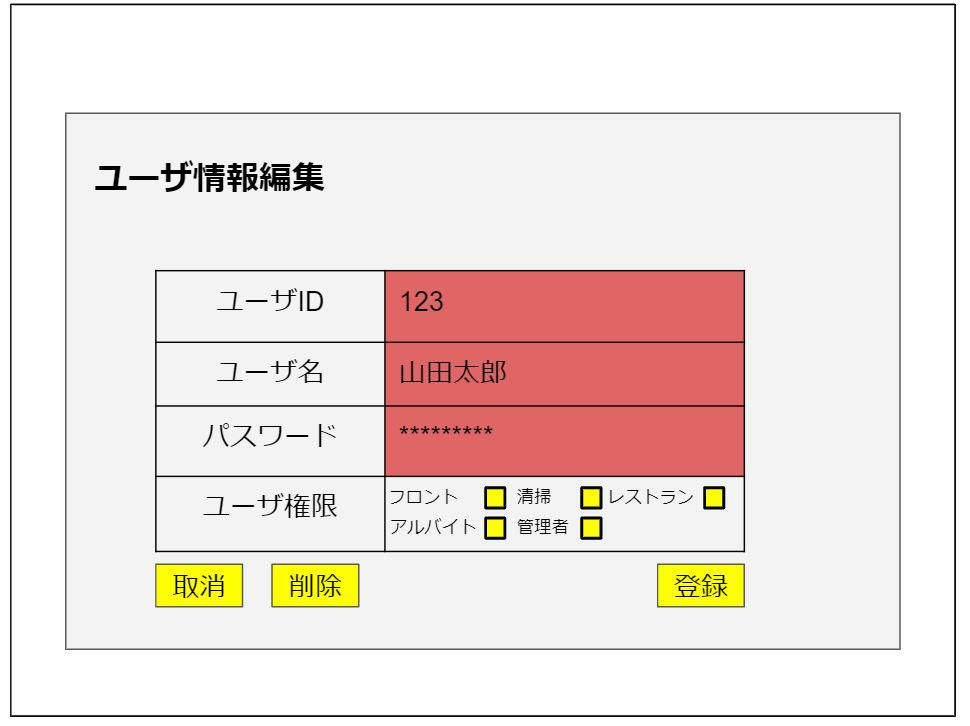
\includegraphics[width=7cm]{UI-umino/user3.JPG}
        \caption{ユーザ情報編集画面}
        \label{fig:user3}
    \end{minipage} 
\end{figure}

\subsubsection{変更・削除確認画面}
図\ref{fig:user4}にユーザ情報変更確認画面,図\ref{fig:user5}にユーザ情報削除確認画面を示す.戻るをクリックすることで図\ref{fig:user4}または図\ref{fig:user5}に遷移する.確定をクリックし,処理が正常に行われた場合には図\ref{fig:user6}に遷移する.エラーが発生し処理が行えなかった場合には図\ref{fig:user7}に遷移する.

\begin{figure}[H]
    \begin{minipage}{0.5\hsize}
        \centering
        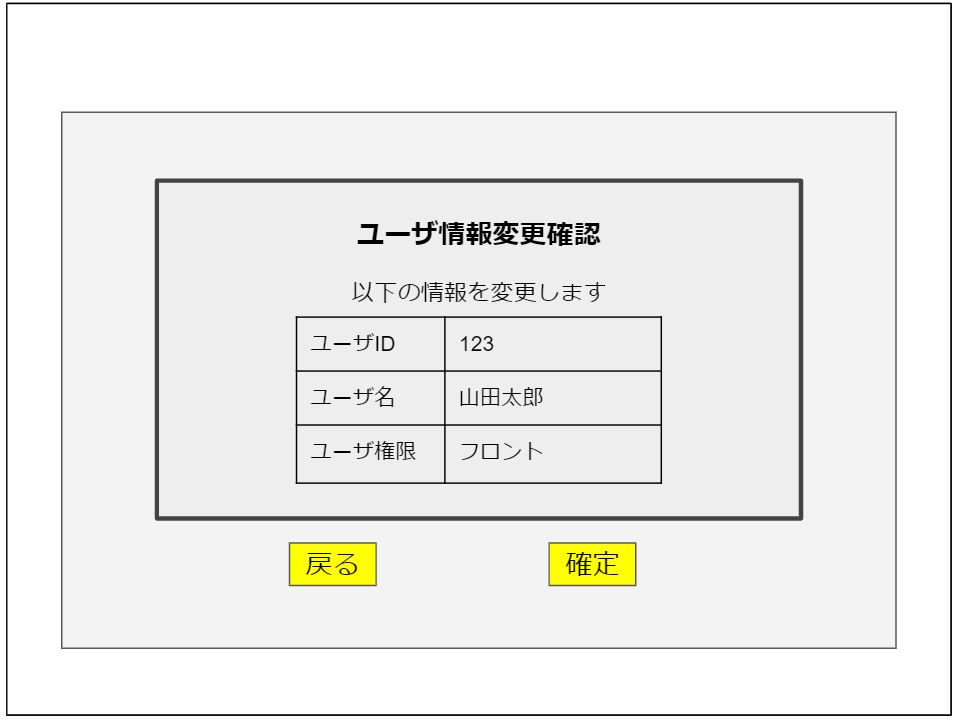
\includegraphics[width=7cm]{UI-umino/user4.JPG}
        \caption{ユーザ情報変更確認画面}
        \label{fig:user4}
    \end{minipage}
    \begin{minipage}{0.5\hsize}
        \centering
        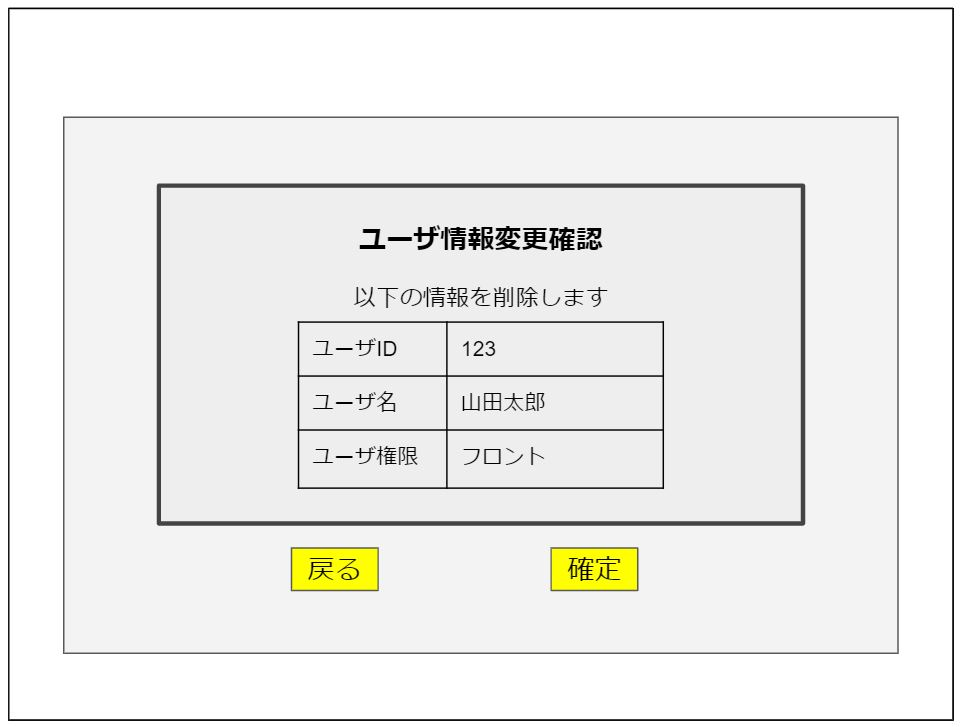
\includegraphics[width=7cm]{UI-umino/user5.JPG}
        \caption{ユーザ情報削除確認画面}
        \label{fig:user5}
    \end{minipage} 
\end{figure}

\subsubsection{変更完了・エラー画面}
図\ref{fig:user6}に正常にユーザ情報の変更が行えた場合の完了画面,図\ref{fig:user7}に正常な処理が行えなかった場合のエラー画面を示す.ユーザ情報管理画面へをクリックすることでどちらも図\ref{fig:user1}に遷移する.

\begin{figure}[H]
    \begin{minipage}{0.5\hsize}
        \centering
        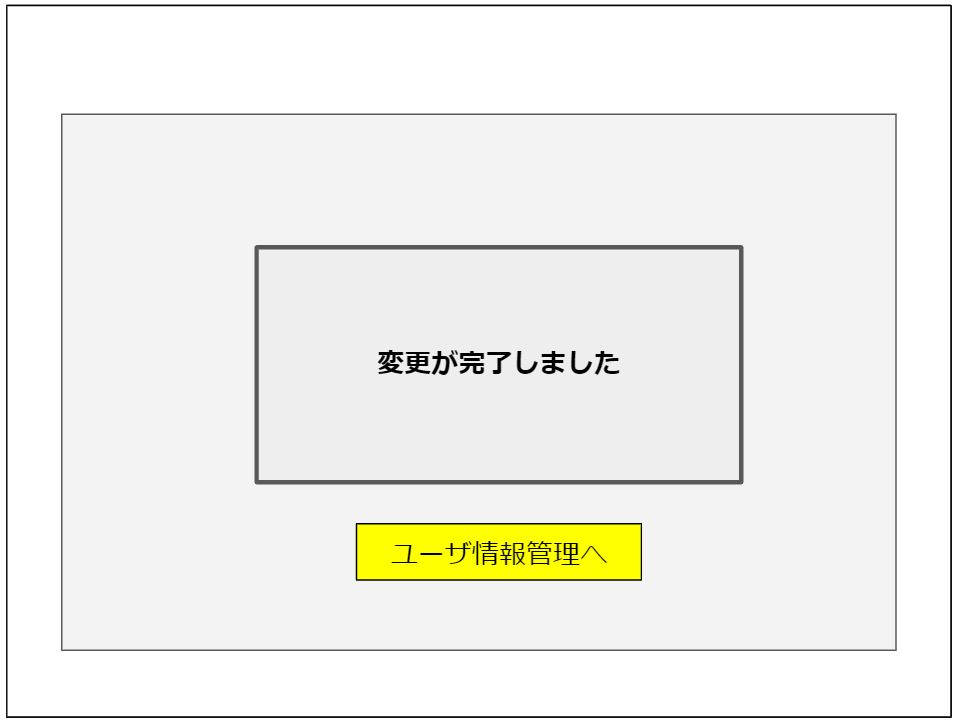
\includegraphics[width=7cm]{UI-umino/user6.JPG}
        \caption{ユーザ情報変更完了画面}
        \label{fig:user6}
    \end{minipage}
    \begin{minipage}{0.5\hsize}
        \centering
        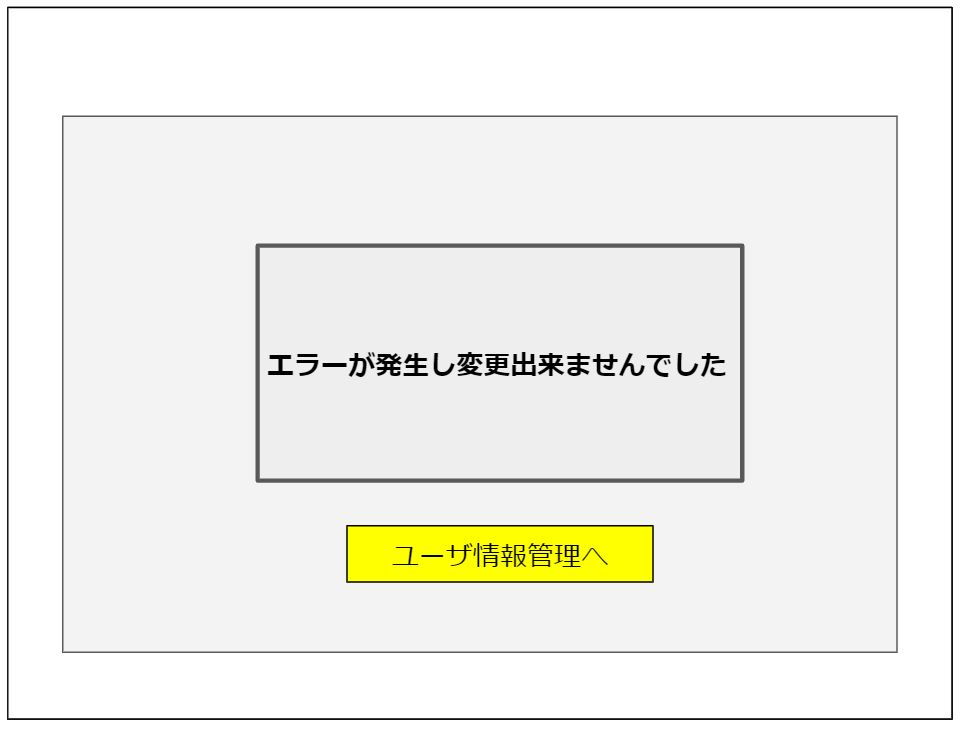
\includegraphics[width=7cm]{UI-umino/user7.JPG}
        \caption{ユーザ情報変更エラー画面}
        \label{fig:user7}
    \end{minipage} 
\end{figure}

\subsubsection{システムログ参照画面}
図\ref{fig:log}にシステムログ参照画面を示す.表示する内容は表\ref{fig:data_log}のデータである.日時を対象として昇順降順を選択できる.TOPへ戻るをクリックすることで図\ref{fig:TOP1}に遷移する.

\begin{figure}[H]
 \centering
   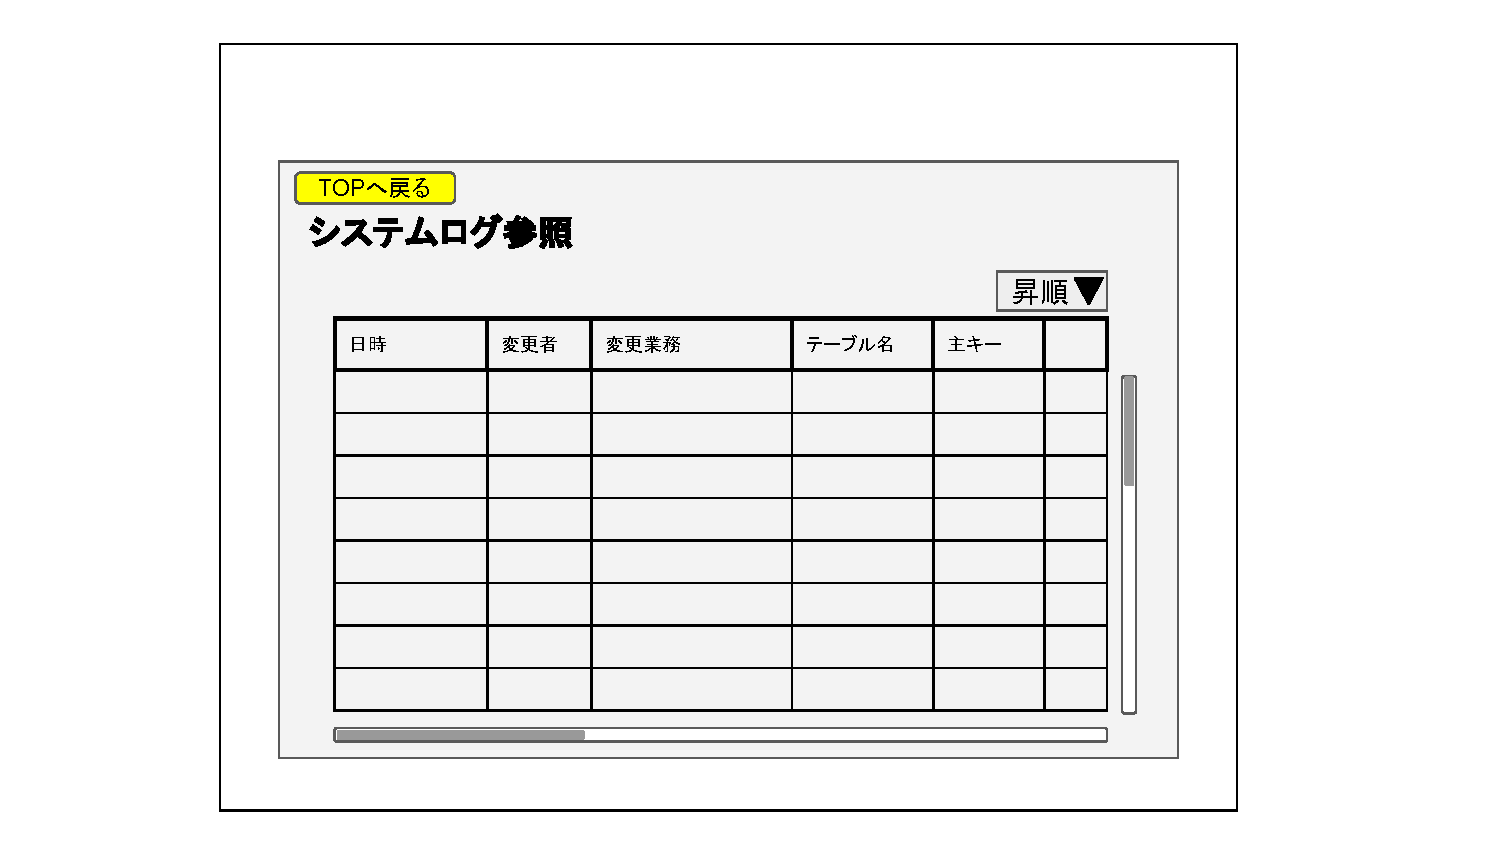
\includegraphics[width=150mm]{UI-umino/system-log-preference.pdf}
 \caption{システムログ参照画面}
 \label{fig:log}
\end{figure}

\subsubsection{よくある質問管理画面}
図\ref{fig:que1}によくある質問管理画面を示す.機能は図\ref{fig:user1}のユーザ情報管理画面と同じく,質問の新規入力と質問の編集が行える.

\begin{figure}[H]
 \centering
   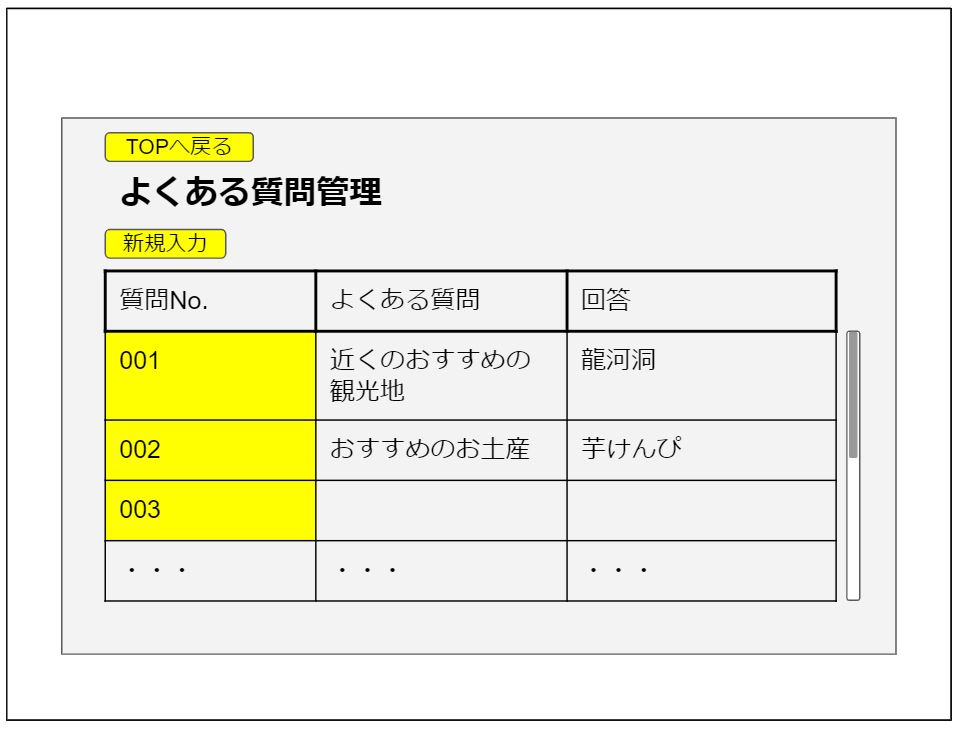
\includegraphics[width=100mm]{UI-umino/que1.JPG}
 \caption{よくある質問管理画面}
 \label{fig:que1}
\end{figure}

\subsubsection{質問情報入力・編集画面}
図\ref{fig:que2}に新規質問入力画面を,図\ref{fig:que3}に質問情報編集画面を示す.質問Noは自動で振り当てられる.質問内容,回答,備考はユーザがキーボード入力を行う.取消をクリックすることで図\ref{fig:que1}に遷移する.削除と登録をクリックすることで図\ref{fig:user4}や図\ref{fig:user5}と同じ様式の画面に遷移し,そこから図\ref{fig:user6}や図\ref{fig:user7}と同じ様式画面に遷移する.

\begin{figure}[H]
    \begin{minipage}{0.5\hsize}
        \centering
        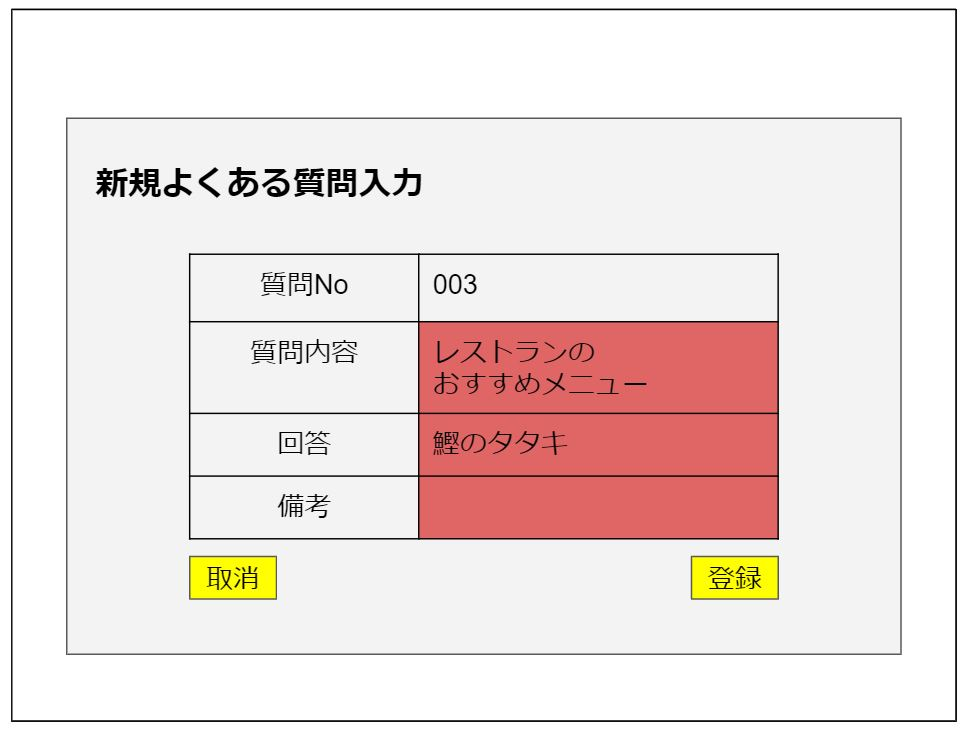
\includegraphics[width=7cm]{UI-umino/que2.JPG}
        \caption{新規質問入力画面}
        \label{fig:que2}
    \end{minipage}
    \begin{minipage}{0.5\hsize}
        \centering
        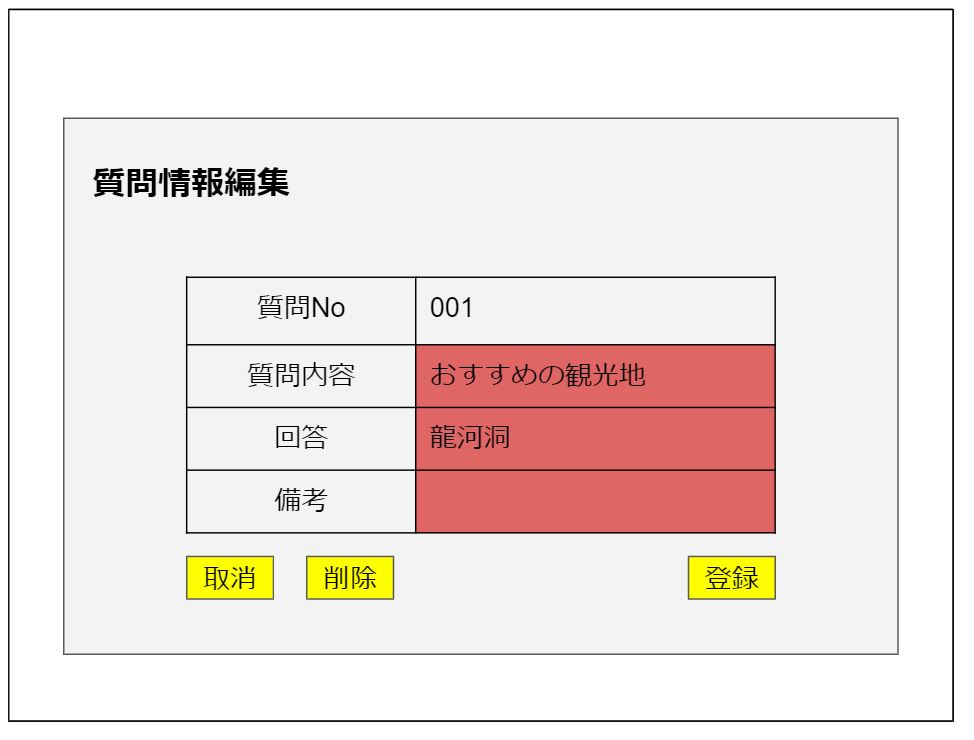
\includegraphics[width=7cm]{UI-umino/que3.JPG}
        \caption{質問情報編集画面}
        \label{fig:que3}
    \end{minipage} 
\end{figure}

\subsubsection{マニュアル情報管理画面}
図\ref{fig:manyu1}にマニュアル情報管理画面を示す.機能は図\ref{fig:user1}と同じく,マニュアルの新規入力とマニュアルの編集が行える.

\begin{figure}[H]
 \centering
   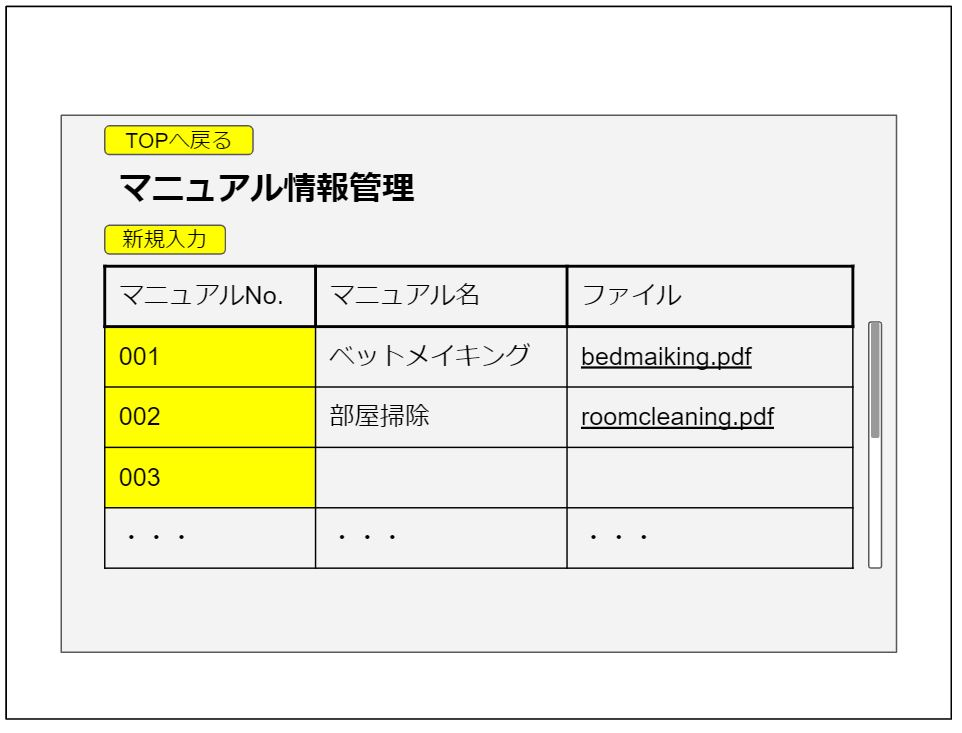
\includegraphics[width=100mm]{UI-umino/manyu1.JPG}
 \caption{マニュアル情報管理}
 \label{fig:manyu1}
\end{figure}

\subsubsection{マニュアル情報入力・編集画面}
図\ref{fig:manyu2}に新規マニュアル情報入力画面,図\ref{fig:manyu3}にマニュアル情報編集画面を示す.マニュアルNoは自動で割り当てられる.マニュアル名と備考はユーザがキーボード入力を行う.表示するファイルはユーザがアップロードする.取消,削除,登録をクリックした際の処理はユーザ情報や質問情報入力・編集画面と同様である.

\begin{figure}[H]
    \begin{minipage}{0.5\hsize}
        \centering
        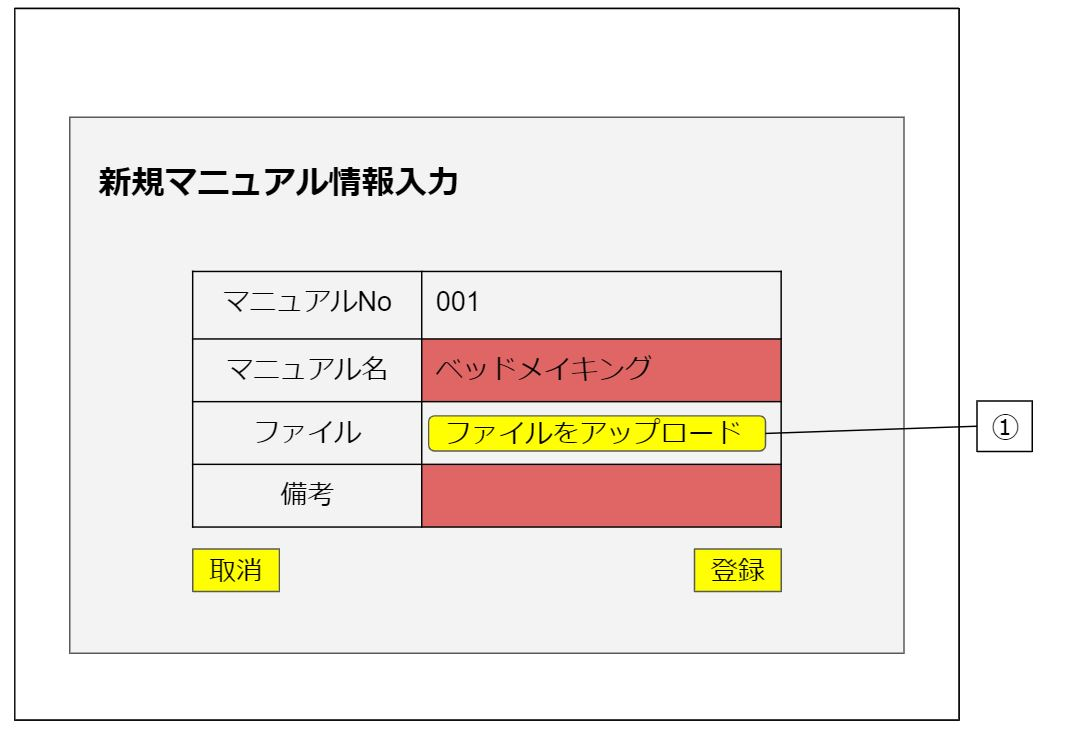
\includegraphics[width=7cm]{UI-umino/manyu2.JPG}
        \caption{新規マニュアル情報入力画面}
        \label{fig:manyu2}
    \end{minipage}
    \begin{minipage}{0.5\hsize}
        \centering
        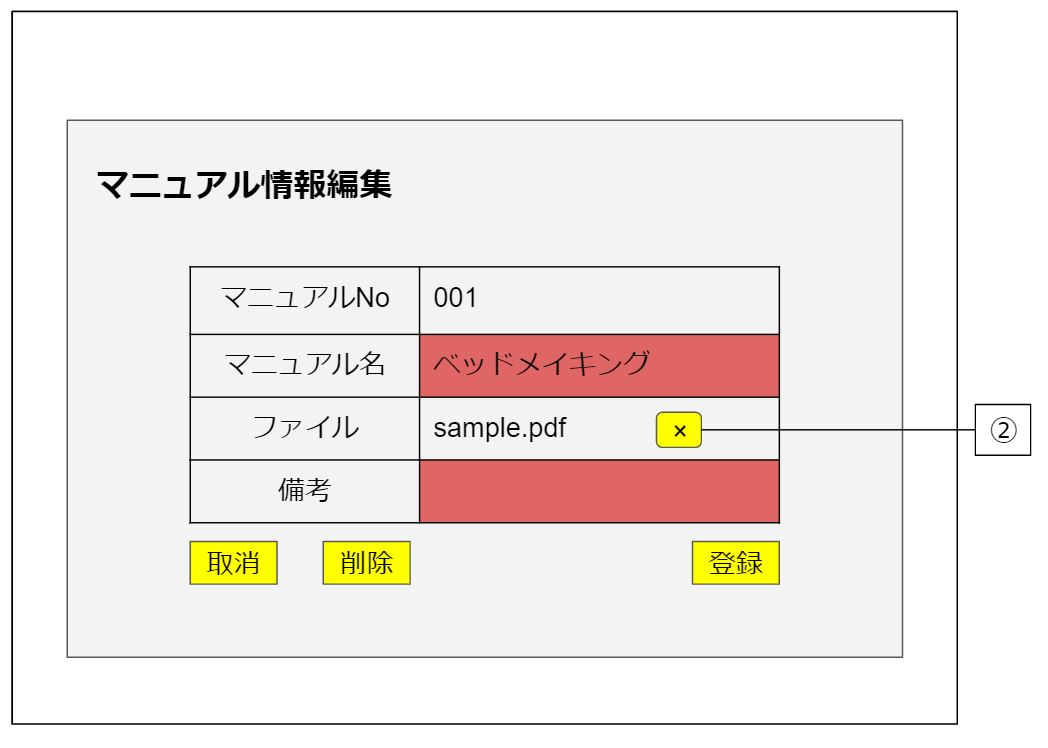
\includegraphics[width=7cm]{UI-umino/manyu3.JPG}
        \caption{マニュアル情報編集画面}
        \label{fig:manyu3}
    \end{minipage} 
\end{figure}

\begin{enumerate}
\renewcommand{\labelenumi}{\textcircled{\scriptsize \theenumi}}
\item ファイルのアップロード\\ クリックすることで端末内からファイルを指定してアップロードすることができる.
\item ファイルの削除\\ バツ印をクリックすることですでにアップロードされているファイルを削除することができる.

\end{enumerate}

\end{document}